\chapter{Tvorba edukačných materiálov} 
Súčasný stav problematiky tvorby edukačných materiálov obsahuje zákonitosti stavby a funkcií učebnice, odporúčania pri písaní zrozumiteľných učebných textov a rozvrhovaní didakticky správneho systému úloh v zbierke. Tiež porovnáme doterajšie učebnice programovania pre stredné školy navzájom a vzhľadom na štátny vzdelávací štandard. 

\section{Učebnica}
Základným prameňom poznatkov a nositeľom obsahu vzdelávania je učebnica, ktorá patrí medzi čelných predstaviteľov pedagogických textov. Predstavuje jadro zoskupujúce okolo seba ostatné učebné prostriedky (\cite{zujev_ako_1986}). V medziach učebných osnov vymedzuje obsah základného učiva s doplnením o rozširujúce učivo, pričom rozsah osnovy učebnice nemusí byť totožný s učebnými osnovami (\cite{mlady_tvorba_1988}). 

Učebnica pomáha žiakom s osvojením si obsahu učiva, čím podporuje všetky súvisiace čiastkové činnosti: precvičovania, opakovania, systematizácie a integrácie. V edukačnom procese učebnica pôsobí aj výchovne, čím vplýva na formovanie postojov, motívov a záujmov. Odlišuje sa v tom od iných kníh a texov, pretože má priamu spätosť so získavaním a spracovaním faktov, pojmov a vzťahov žiakmi. Efektívne tak smeruje dosiahnutie výchovno-vzdelávacích cieľov vyučovacieho predmetu (\cite{gavora_ziak_1992}). Učebný program žiaka a vyučovací program učiteľa je ideálne v učebnici pochytený a odráža sa do scenáru učebného a vyučovacieho procesu. Hlvaná časť učebnice prestavuje súbor úloh určených na aktívne riešenie (\cite{pavlovkin_ziak_1989}).

Podľa školského zákona sa učebnica spolu s učebným textom a pracovným zošitom zaraďuje medzi edukačné publikácie. Na vzdelávanie sa používajú edukačné publikačné schválené ministerstvom školstva alebo zodpovedajúce princípom a cieľmi výchovy a vzdelávania (\cite{skolsky_zakon}). Princípy súvisiace s vlastnými vzdelávacími materiálmi sú v duchu rovnoprávnosti, rovnocennosti, zodpovednosti, tolerancie a vyváženého rozvoja osobnosti a zdokonaľovania vzdelávania podľa výsledkov výskumu a vývoja.

\subsection{Didaktické funkcie učebnice}
V učebnici pôsobí viacero naviazných a prelínajúcich sa vlastností vystupujúcich vo výchovno-vzdelávacom procese (\cite{zujev_ako_1986}), ktoré sú popísané bez stanoveného poradia dôležitosti:
\begin{itemize}
\itemsep0pt
\item \textbf{Informačná funkcia}: sa sústreďuje na stanovenie povinného rozsahu informácií pri štúdiu nevyhnutných na zapamätanie.
\item \textbf{Transformačná funkcia}: spočíva v didaktickom transfere poznatkov vedného odboru na obsah učiva v zrozumiteľnej a pútavej podobe, a zaroveň sa berie do úvahy na vekové a kultúrne osobitosti žiakov. Nabáda na výber vzdelávacích metód a uľahčuje aktivizáciu žiaka pri cvičeniach a úlohách prieskumného charakteru. Pri transformácii znalostí sa hľadí sa aj na potreby profesijného života a spoločenského očakávania od absolventov.
\item \textbf{Systematizačná funkcia}: pri objasňovaní učiva zabezpečuje následnosť poznatkov, postupný nárast náročnosti a vedie k metódam vedeckej systematizácie.
\item \textbf{Usmerňujúca funkcia}: slúži k upevňovaniu vedomostí napomáha v orientácii sa v nich a zapojením ich do praktických druhov činností. Vyžaduje sprevádazanie navrhnutými aktivitami pod vedením učiteľa.
\item \textbf{Motivačná funkcia}: pobáda túžbu a schopnosti žiakov na samostatné získavanie vedomostí.
\item \textbf{Integračná funkcia}: ucelene spája poznatky žiakov nadobudnuté z ich rozličných činností.
\item \textbf{Koordinačná funkcia}: zapája ku vzťahu k študovanému predmetu informácie z masovo-komunikačných prostriedkov. 
\item \textbf{Výchovná funkcia}: súčasne tiež rozvíjajúca funkcia, ktoré spočívajú v zladenom formovaní čŕt osobnosti žiaka.
\end{itemize}
Uvedené didaktické funkcie zabezpečujú komplexné pôsobenie učebnice na rozvoj kognitívnych a afektívnych schopností žiaka. Pri ich prepojení v učebnom texte dochádza nielen k nadobudnutiu nevyhnutných vedomostí a zručností na zvládnutie vyučovacieho predmetu, ale aj rozvoj kľúčových kompetencií a medzi nimi pripravenosti k všestrannejšiemu učeniu sa.


\subsection{Prvky učebnice}
Aby učebnica plnohodnotne napĺňala svoje mnohé poslania je poskladaná z \textbf{prvkov textového i mimotextového charakteru}, ktoré podnecujú aktívne kognitívne procesy a umožňujú zapojenie zvoleného učebného štýlu čitateľa. Zaradenie súčastí učebnice do členenia jej podsystémov nie je striktné, ale riadi sa dominantnou funkciou danej časti (\cite{zujev_ako_1986}).

Text v učebnici je súhrn viacerých viet, ktoré sú prostriedkom na odovzdanie informácií žiakom podľa komunikačného zámeru autora. Z povahy súvislého písaného jazykového prejavu sa vyznačuje kohéziou a koherenciou. Kohézia je súdržnosť textu na úrovni vzájomnej nadväznosti medzi vetami za použitia gramatických, lexikálnych a grafických jazykových prostriedkov. Najčastejšie sa uplatňujú gramatická zhoda medzi nadradeným a podradeným slovným druhom alebo vetným členom, opakovanie výrazu ďalej v texte, synonymá, a interpunkčné znamienka. Koherencia je zase tématická spojitosť textu, keď sa z hlavnej rozvíjajú vedľajšie myšlienky   (\cite{gavora_ziak_1992}). 

Podľa úlohy, ktorú zohráva text v predstavovaní učebnej látky sa rozlišuje \textbf{základný, doplňujúci a vysvetľujúci text}. Základný text je určený ako povinný na osvojenie pre zvládnutie problematiky. Podľa typu činností motivovanej základným textom sú povšimnuté teoretické poznávacie texty považované tiež za výkladovú zložku zastávajúcu informačnú funkciu vysvetľovania a komentovania nového učiva. Kdežto u inštrumentálno-praktických textov, alebo aj nevýkladovej zložky prevláda transformačná funkcia premietajúca sa do otázok, úloh a cvičení. Doplňujúci text prehlbuje rozsah učebných osnov dodatočňou argumentáciu vplývajúcej na rozumovú a emočnú stránku. Regulovanie poznávacej činnosti má na starosti vysvetľujúci text, ktorý dáva základný text do súvislostí (\cite{zujev_ako_1986}).

Mimotextové zložky nachádzajúce sa v učebnici sú zatrieďované na \textbf{aparát organizácie osvojovania, ilustračný materiál, a orientačný aparát}. Na organizáciu osvojovania slúžia prehľadové tabuľky, otázky a úlohy spolu s odpoveďami, ktoré v závislosti od kontextu sú spadajú do základného textu. Ilustrácie prevažne graficky dotvárajú textovú zložku, s ktorou sú vo vzťahovej rovine buď nadradenosti ako vedúce ilustrácie, rovnocennosti, alebo podradenosti ako doplnkové ilustrácie. Súvislosť medzi textom a ilustráciou sa spozná, podľa toho či text opisuje ilustráciu, vtedy je text podradený, alebo ilustrácia slúži na dokreslenie sitúcie. Typickými príkladmi ilustrácií sú obrázky, schémy, plány, diagramy, grafiky, mapy. Orientačný aparát slúži na zdôraznenie slovných spojení alebo myšlienok cez tlačové zvýraznenia a symbolické značenie, alebo opakuje prvky z hlavnej časti v zhutnenej podobe na navigáciu v knihe, v čom spočíva úloha napríklad predhovoru, obsahu, a registrov (\cite{zujev_ako_1986}).

Tradičná redakčná výroba učebnice dbá na ustálené metódy a organizovanú spoluprácu pre kontrolu správnosti obsahu po odbornej stránke a dohliada na gramatickú, pravopisnú a štylistickú úpravu (\cite{mlady_tvorba_1988}). Zasadzuje sa o koordináciu činnosti autorských kolektívov, tak aby umožnila zosúladiť všetky dôležité prvky učebnice najmä však súhru textovej a grafickej časti. Osvedčené pracovné postupy redakcie zabezpečujúce zahrnutie podstatných zložiek učebnice začínajú vypracovaním jej osnovy, príprave materiálov a podkladov, následne príprave rukopisu a obrazových predlôh v čase vymedzenom stanoveným harmonogramom, ktoré prechádzajú korektúrou, a celkové snaženie je zavŕšené vydaním učebnice a získaním doložky ministerstvom školstva podľa osobitého predpisu. Tvorba vzdelávacích materiálov priamo učiteľmi nie je až tak rigidná, ale navádza na zmysluplnú organizáciu práce.

\subsection{Multimediálne prostredie}
Postavenie výuky informatiky okolo počítačov a súvisiaceho prídavného vybavenia vedie k prirodzenej snahe uspôsobovať edukačné materiály naskýtajúcim sa podmienkam. Tým môžu učebné texty zúžikovať príležitosti pre obohatenie ich obsahu multimédiami a hypertextovými prepojeniami. Princípy uplatňujúce sa pri tvorbe klasických učebníc sa nevyhnutne prenášajú aj na tvorbe multimediálnych učebníc, pretože rovnako zostávajú publikáciami uspôsobených ku didaktickej komunikácii (\cite{krotky_nove_2015}).

Množstvo existujúcich učebníc prechádza do online prostredia zo svojej pôvodne knižnej úpravy na zvýšenie ich atraktívnosti a pohodlia pri prístupe k nim. Ani vznik učebnice určenej primárne pre elektronické médium však ešte nezaručuje využitie ponúkaného potenciálu na skĺbenie inovatívnych vyučovacích metód a ponúknutých technických vymožeností. Preto sa odlišujú učebnice podľa náročnosti prítomných konštrukcií na \textbf{jednoduché, komplexné a pokročilé učebnice} (\cite{krotky_nove_2015}).

Jednoduché učebnice sú elektronické obrazom svojich papierových vzorov bez uplatnenia akýkoľvek nových rozširujúcich možností. Komplexné učebnice získame zakomponovaním multimediálnych prvkov, zastúpených prevažne zvukmi, obrázkami, animáciami, videom, a vložením  hypertextových odkazov smerujúcich dovnútra vlastného obsahu a na externé webové portály a ďalší multimediálny obsah. Pokročilé učebnice navyše pozostávajú s interaktívnych prvkov aktívne prispôsobujúcich tok informácii a manipulácie s nimi cez tlačidlá, posuvníky kontextové nápovedy, a príbuzné ovládanie. Nadstavbou pokročilej učebnice je edukačný softvér.

\subsection{Skvalitňovanie učebného textu}
Vylepšenia v učebných textoch sa uskutočňujú na základe teoretických východísk z porozumeniu textu pri \textbf{čítaní ako psycholingvistickej činnosti}. Na úspešné odhalenie komunikačného zámeru pozná recipient vzťah medzi objektívnou realitou a na ňu odkazujúce prvky textu, medzi jednotlivými prvkami textu a medzi textom a doterajšími znalosťami prijímateľa (\cite{gavora_ziak_1992}). 

Práve operáciou elaborácie sa nachádzajú asociácie v prečítanom texte s už nadobudnutým sémantickými a epizodickými znalosťami a vizuálnymi predstavami, pokiaľ existuje také spojenie. Inferencia umožňuje doplnenie zamlčaných informácii v texte, ktoré vyplývajú z opísaných pričinno-dôsledkových súvislostí (\cite{gavora_ziak_1992}).

Počas zvnútorňovania edukačného textu dochádza k postupu od jeho porozumenia bez vzťahu k iným textom, cez prevod na parafrázy a symbolický zápis, cez interpretáciu vnášajúcej odlišný pohľad na prečítané, až ku extrapolácii inovatívnych záverov a schopnosti predpovedať dôsledky (\cite{gavora_ziak_1992}). 

Na objasnenie nových konceptov je teda prospešné, ak sú úvadzané východiskové situácie povedomé a autorova predstava sa zhoduje s čitateľovou. Čítaním môže nastať neporozumenie v tzv. \textbf{mikroštruktúre textu}, to sú slová, vety, vzťahy medzi vetami, či štruktúra textu. Neznámym slovám dokážeme predchádzať ich vhodným výberom usúdenej z náročnosti pojmu. Taxonomické normy zachytávajú typickosť pojmov, tým že ho spájajú s názvom nadradenej kategórie. Zložité vety odkazujúce sa vedľajšou vetou na vzdialené slová a včlenené prívlastkové vety by mali byť radšej rozdelené na dve vety. Pozornosť treba venovať neopomenutiu podstatných spájajúcich slov. 

\textbf{Zložitosť textu} sa opisuje kvantitatívnymi charakteristikami, prejavujúce sa v čitateľnosti a náročnosti texu. \textbf{Čitateľnosť} sa zvykne merať dĺžkou viet alebo výskytom neobvyklách slov. Jednou z mnohých mier čitateľnosti je Gunning \emph{Fog index} v prijateľnom rozsahu pre stredné školy do skóre 14 (Vzorec~\ref{equ:fog-index}) (\cite{drahosova_hodnotenie_2014}). 

\textbf{Náročnosť} textu vychádza z lexikálnych a syntaktických faktorov, ktoré pokladajú na škálu zložitosť toho čo je povedané a akým spôsobom je to zapísané. \emph{Průchová modifikácia Nestlerovej metódy} zisťuje obtiažnosť na vzorkách výkladového textu učebnice zohľadnením syntaktickej a sémantickej náročnosti  v bodovom rozpätí pod 20 bodov (nízka obtiažnosť) a nad 60 bodov (vysoká obtiažnosť) (Vzorec \ref{equ:nestler-method}) (\cite{drahosova_hodnotenie_2014}). Textu vyjadrujeme tiež inferenčnú záťaž, teda nutnosť vyvodzovania vzťahov čitateľom, sa znižuje umiestnením podobných myšlienok za sebou (\cite{pavlovkin_ziak_1989}).

\begin{ceqn}\begin{align}
0.4 \cdot \left(\left(\frac{\sum slova}{\sum vety}\right) + 
\left(\frac{\sum \text{slova nad 2 slabiky}}{\sum slova}\cdot 100\right)\right)
\label{equ:fog-index}
\end{align}\end{ceqn}

\begin{equation}\begin{split}
& 0.1 \cdot \left(\frac{\sum slova}{\sum vety}\right) \cdot  \left(\frac{\sum slova}{\sum slovesa}\right) + \\
& \left(\frac{\sum pojmy}{\sum slova}\right) \cdot \left(\frac{\sum P_1 + 3\sum P_2 + 2\sum P_3 + 2\sum P_4 + \sum P_4}{\sum slova}\right)
\label{equ:nestler-method}
\end{split}\end{equation}

Ku kvalite textov učebnice prispieva aj \textbf{makroštruktúra textu}, čiže rozčlenenie tématických okruhov na kapitoly a tie na texty. Na poskytnutie nadhľadu slúžia typografické zvýraznenia hrubým písmom alebo oddeľujúcim práznym priestorom, nadpisy rôznych veľkostí na rozlíšenie tém a podtém, kľúčové vety vyjadrujúce hlavnú myšlienku, a uvádzajúce či rekapitulúce otázky pobádajúce čiateľa na aktívne prijímanie materiálu (\cite{pavlovkin_ziak_1989}). Nemenej znateľná pri čítaní je primerane jednoduchá grafická úprava neodpútavajúca pozornosť od obsahu. Prehľadnosť sa vylepšuje nastavením ľahko čitateľného písma s veľkosťou odrážajúcou hierarchiu celkov, riadkovaním do bloku, a zalamovaním príkladov v celku na jednu stranu (\cite{mlady_tvorba_1988}).

Na hodnotenie kvality učebníc sa uplatňujú experimentálne, expertné a štatistické metódy. V autentickom školskom prostredí môžeme experimentálne overovať a porovnávať navrhovanú učebnicu so staršou zaužívanou. Pozorovatelia učebnice ako sú experti, učitelia a žiaci hodnotia rozličné vlastnosti s ktorými prichádzajú do kontaktu, napríklad primeranosť, metodické spracovanie, zaujímavosť, zložitosť. Štatisticky sa kvantifikuje rozsah textu určený na vyučovaciu jednotku, čitateľnosť a náročnosť textu.

Výskum Drahošovej sumarizuje nasledujúce techniky pre pedagogickú prax na zlepšovanie zrozumiteľnosti učebného textu. Ohľadom výberu slov odporúča uprednostniť bežné slová, opísateľné pojmy a aktívne slovesá, zároveň sa vyhýbať nepotrebným slovám. V rovine štylistiky by sa malo písať s priblížením sa bežne hovorenej reči, v jednduchých celkoch a krátkych vetách. Myšlienky textu vyjadrovať adresne a presvedčivo s opieraním o skúsenosti čitateľa (\cite{drahosova_hodnotenie_2014}).

\section{Systém úloh v zbierke}
Skupina úloh sa označuje systémom úloh, keď plní konkrétnu didaktickú funkciu v súlade s učebnými cieľmi, štruktúrou poznávacieho procesu a podmienkami učebného procesu sa označuje systém úloh (\cite{mindakova_tvorba_2008}). Otázky na precvičovania učiva sa vyznačujú špecifikami oproti výkladovému textu, prevažne tým že ich vyriešenie bezpochyby vyžaduje aktívnu činnosť žiaka na rôznych úrovniach myslenia. Učiteľ v tomto štádiu pozoruje postup žiakov pri vypracovaní úloh a na základe ich vonkajších prejavov posudzuje a usmerňuje ich činnosť k želanému cieľu. Kritické je stanoviť následnosť a hierarchiu úloh, tak aby umožňovali kontinuálny rozvoj žiaka. V teminológii B.~F.~Skinnera vyvinúť program výučby.   

\subsection{Psychologické východiská}
Návrh systému úloh sa potýka s otázkami žiackej motivácie riešenia úloh, diferenciácie úloh vzhľadom na individuálne osobitosti žiakov, vhodného zoradenia úloh od jednoduchších k zložitejším a spôsobu merania stupňa zvládnutia učiva. Nie je očakávateľné, že všetky témy budú samy osebe atraktívne. Dieťa sa však aspoň odhodlá k takým úlohám, ktoré sa domnieva že prekoná bez pociťovaných obtiaží. Úspech prirodzene motivuje na skúšanie väčších výziev a nepríjemné skúsenosti a zlyhanie odrádzajú. 

Výber a zoradenie úloh má zaručiť zážitky úspechu. Primeraný cvičebný materiál zodpovedá poznávaciemu potenciálu dieťaťa vo \textbf{vekových osobitostiach, individuálnych odlišnostiach a predchádzajúcich skúsenostiach}. Pokrok v psychickom vývine vyšších schopností dosiahneme zaradením nielen veku primeraným problémov, ale aj rozvíjajúcich pre rozšírenie zóny najbližšieho vývinu podľa S.~L.~Vygotského. Z hľadiska individuálnych predpokladov na riešenie úlohy sa treba zamýšľať nad optimálnymi poznávacím štýlom, celkovou úrovňou schopností a profilom schopností na splnenie konkrétneho zadania. V zbierkach sa preto ponúkajú úlohy troch úrovní náročnosti: \textbf{menej náročné, stredné, vysoko náročné}~(\cite{pavlovkin_ziak_1989}).
 
Skupinu menej náročných úloh vedia riešiť priemerní žiaci v nižšom ročníku, teda sú určené na opakovanie a pre žiakov s pomalším tempom vývinu či nižšou poznávacou kapacitou. Stredne náročné úlohy s najväčšou početnosťou sú pochopiteľné pre priemerných žiakov v danom ročníku. Žiaci s vyššou poznávacou kapacitou dokážu prejsť vysoko náročnými úlohami, ktoré sú určené pre priemerných vo vyššom ročníku.
 
Úlohy by mali byť prispôsobené okrem schopností žiaka aj vedomostiam a spôsobilostiam. Získavanie nových schopností prechádza od nadobudnutia vedomostí v podobe pojmov a schém, cez osvojovanie spôsobilostí v priebehu čoraz vyladenejšieho motorického, senzomotorického a psychického cvičenia, až k rozvíjaniu myslenia spojeného s stratégiami formulácie problému a plánovania riešenia~(\cite{pavlovkin_ziak_1989}).

Efektívneho učenia celkove dosiahneme podľa Skinnera, keď sú známe konkrétne ciele výchovy a vzdelávania, žiakom je umožnené postupovať vlastným tempom nezávisle na ostatných a okamžitou spätnou väzbou s odhalením správnej odpovede~(\cite{pavlovkin_ziak_1989}).


\subsection{Klasifikácia vlastností úlohy} \label{sec:klasifikacia-ulohy}
Naplnenie tématického celku náročnosťou odstupňovaními úlohami s rozmanitými didaktickými funkciami a zapojením kognitívnych funkcií naprieč úrovňami myšlienkových operácií sa dá skontrolovať cez špecifikáciu vlastností konkrétnej úlohy. Od charakteristík úlohy sa odvíja  jej zaradenie do zbierky a sú to (s príkladmi z matematiky)~(\cite{mindakova_tvorba_2008}):

\begin{itemize}[noitemsep]
\item \textbf{Téma}: názov tématického celku vo vyučovacom predmete \emph{(napr. Funkcia)}.
\item \textbf{Podtéma}: téma sa rozdeľuje na viaceré časti \emph{(napr. Lineárna funkcia, \dots)}
\item \textbf{Element}: pojmy, vzťahy a procesy podľa obsahového štandardu. Rozsiahlejšie elementy môžu vystupovať ako podtémy \emph{(napr. Pytagorova veta)}
\item \textbf{Funkcia}: didaktické požiadavky na poznávací proces. Prípustné je ak úloha napĺňa niekoľkých didaktických funkcií (napr. slovná úloha na upevnenie učiva s aplikáciou poznatkov mimo matematiky). Úlohy na základe didaktickej funkcie podľa D.~Švedu sú (\cite{sveda_ulohy_1992}):
\begin{enumerate}[label=\alph*),noitemsep,topsep=0pt]
\item úlohy na motiváciu učebnopoznávacej činnosti žiakov
\item úlohy na aktualizáciu skôr osvojeného učiva
\item prípravné úlohy predchádzajúce vysloveniu definície pojmu a riešeniu základných úloh 
\item úlohy na osvojenie definície pojmu, formulácie vety a postupu riešenia
\item úlohy na upevňovanie učiva
\item úlohy na aplikáciu učiva mimo informatiky
\item úlohy na aplikáciu učiva vo vnútri informatiky
\item úlohy propedeutického charakteru k nasledujúcim elementom učiva v tematickom celku
\item úlohy na opakovanie a systemizáciu
\end{enumerate}

\item \textbf{Úroveň}: úloha rozvíja zároveň všetky nižšie úrovne poznávacích procesov, preto sa označuje iba najvyššou. Poznávacie procesy podľa M.~Zelinu sú (\cite{zelina_tvorivost_1990}):
\begin{enumerate}[label=\alph*),noitemsep,topsep=0pt]
\item vnímanie
\item pamäť
\item nižšie konvergentné procesy
\item vyššie konvergentné procesy
\item hodnotiace myslenie
\item tvorivé, divergentné myslenie
\end{enumerate}
\end{itemize}

Klasifikácia úlohy podľa uvedených kritérii je náročná a subjektívna, lebo pri zaradení záleží od mnohých okolností ako sú formulácia úlohy, vedomosti a skúsenosti žiakov, podmienok vyučovania a organizačného prístupu učiteľa (\cite{mindakova_tvorba_2008}). 

\subsection{Preformulovávanie úloh}
Často sa vyskytujúci nedostatok systému úloh je neúplnosť pestrosti didaktického zamerania cvičení. Ukázalo sa, že nedostatok úloh vo fáze aktualizácie učiva, v prípravnej fáze alebo vo fáze osvojovania učiva sa dá prekonať vytvorením nových úloh vo forme jednoduchých otázok alebo iným zaradením podľa témy, podtémy a elementu učiva. Preformulovaním navyše dosiahneme úpravy kategórii úlohy, či zvýšenie alebo zníženie jej obtiažnosti. Doplnenie chýbajúcich typových úloh sa môže realizovať rozličnými kreatívnymi prístupmi, z ktorých vyzdvihujeme tri systematické metódy (\cite{mindakova_tvorba_2008}):

\begin{enumerate}[label=\alph*),noitemsep,topsep=0pt]
\item \textbf{Zmena podmienky v zadaní}: najčastejšie zmení tému, podtémy, element učiva, čím môže mať vplyv na fáze vyučovacieho procesu, kedy sa úloha osvedčí použiť, napr. z motivačnej na aplikačný typ. Konkrétnosti dopadu na úlohu závisia od presného textu zadania, ale zmeniť podtému úlohy z ,,Príkazy'' na ,,Cyklus'' vieme pridaním požiadavky viacnásobne duplikovať obrazca vedľa seba. Zmenou formátu vstupu programu, z viacerých údajov na jednom riadku rozdelením na viac riadkov, sa úloha dostane z podtémy ,,Reťazce'' do ,,Vstupy programu''.
\item \textbf{Tvorba otočenej úlohy}: poskytuje prelohu na prípravu divergentných úloh, ktoré sú spravidla ťažšie na vymyslenie než na nižšie myšlienkové operácie. V otočeneje úlohe nebudú vyjadrené priamo číslené údaje na dosadenie do vzorca, ale situácia sa ilustuje  graficky a žiak musí zvážiť stratégiu riešenia.
\item \textbf{Zmena fabuly úlohy}: sa spolieha pri sprístupnení podstaty úlohy pre iného adresáta na zmenu príbehu slovnej úlohy a zasadenie do javov do iného kontextu. Nemení umiestnenie úlohy v zbierke. Výpočty o rozmeroch valcovitých predmetov môžu tak nedobudnúť dejovú líniu o bareloch nafty, kmeňoch stromov, stenách rotúnd, alebo elektrickom odpore drôtov.
\end{enumerate}

Vyvážovanie počtu úloh medzi témami a časťami zbierky sa najlepšie dosahuje zmenou podmienky v zadaní. Otvorené úlohy nemajú hojné zastúpenie, pretože zvyknú byť časovo náročné a pre priemerných žiakov za dogmatického spôsobu výučby náročné, najmä tam sa uplatní úprava na obrátenú úlohu. Sady didaktických testov alebo personalizované interaktívne elektronické učebnice, do ktorých je potrebné generovať podobne náročné úlohy z rovnakej oblasti, hojne zúžitkujú zmenu fabuly úlohy.

\section{Vzdelávacie štandardy v informatike}
Výchovno-vzdelávací štadard sú kritéria vzdelávacej inštitúcie na požadovanú úroveň žiakovho výkonu po kognititívnej, formatívnej a konatívnej stránke. Ciele vzdelávania sú predpísané v štátnom vzdelávacom programe \emph{(ŠVP)}, z ktorého školy vychádzajú v školskom vzdelávacom programe \emph{(ŠkVP)}. Tvorí ho obsahový štandard vymedzujúci čo sa má žiak naučiť a výkonový štandard s minimálnou normou činnosti žiaka.

V informatike je ŠVP rozdelený na 5 okruhov: algoritmické riešenie problémov, reprezentácie a nástroje, softvér a hardvér, komunikácia a spolupráca, informačná spoločnosť (\cite{statny_2023}). Konanie internej formy maturitnej skúšky z informatiky nasleduje metodický pokyn cieľových požiadaviek. Dosiaľ sme analyzovali \emph{akým spôsobom} majú učebnice a zbierky úloh predkladať učebnú látku, v súlade so vzdelávacími štandardmi určíme, \emph{čo} majú obsahovať.

\subsection{Algoritmické riešenie problémov}
Algoritmizácia a programovanie reprezentuje až 70\% váhy výslednej známky maturitnej skúšky a najväčší tématický okruh v ŠVP informatiky pre stredné školy, ktorý dostáva v rámcových učebných osnovách ŠkVP najväčší podiel z časovej dotácie až približne tretinu (\cite{cp_2023}). Nemusíme sa pozerať len na formálne dokumenty, aby sme si uvedomili, že programovanie sa stáva v dnešnom technologickom svete a informačnej revolúcii nepostrádateľnou digitálnou kompetenciou pre život.

ŠVP vyčleňuje 8 tématických celkov algoritmizácie (\cite{statny_2023}):
\begin{itemize}[noitemsep,topsep=0pt]
\item \textbf{Analýza problému}: naplánovanie algoritmické riešenie problému rozdelením na menšie časti a opísať ideu v prirodzenom jazyku. Identifikovanie vstupných informácií, očakávaných výstupov a akcií. 
\item \textbf{Jazyk na zápis riešenia}: používanie konštrukcie programovacieho jazyka, vytvárať a interpretovať zápisy podľa pravidiel syntaxe.
\item \textbf{Postupnosť príkazov}: skladanie príkazy do poradia na riešenie probému.
\item \textbf{Nástroje na interakciu}: načítanie neznámej hodnoty na vstupe a zobrazenie výstupu. Ošetrenie prípustného rozsahu alebo formátu hodnôt.
\item \textbf{Premenné}: priradenie do pomenovanej premennej a ich použitie v aritmetike.
\item \textbf{Cykly}: odhalenie repetitívnych vzorov so známym a neznámym počtom opakovaní. Akumulovanie čiastkových výsledkov v tele cyklu a kombinovanie cyklov s vetvením.
\item \textbf{Vetvenie}: stanovenie logickej platnosti vlastnej podmienky obsahujúcej boolovské operácie.
\item \textbf{Interpretácia zápisu riešenia}: odladenie programu krokovaním a opravovanie chýb v existujúcich programoch.
\end{itemize}

Výstižne sa základné pojmy z povinných tématických celkov programovania dajú zhrnúť podľa štruktúr vývojového diagramu na \textbf{sekvenciu príkazov, vstupy, výstupy, podmienky a cykly}. V cieľových požiadavkách na maturitnú skúšku sú témy ešte rozšírené o vnorené príkazy cyklu a vetvenia, \textbf{podprogramy} s parametrami, lokálnými premennými, návratovou hodnotou a nerekurzívnym volaním. Navyše sa pridávajú \textbf{jednorozmerné polia, textové súbory, zložené údajové štruktúry} a použitie \textbf{generátora náhodných čísel} (\cite{cp_2023}).

\subsection{Existujúce učebnice a zbierky úloh}
V prehľade edukačných publikácií, vrátane elektronických, sa upriamime na porovnanie usporiadania uvedenia jednotlivých pojmov, typické formulácie úloh a grafickú úpravu textu. Už učebnica z matematiky pre 3.ročník stredných škol (\cite{sedivy_matematika_1986}) a nadväzujúca zbierka úloh (\cite{busek_zbierka_1987}) z roku 1987 rozoberajú tému algoritmov približne v šírke danej dnešným ŠVP informatiky len s okrajovým doplnením o programovanie v jazyku Basic. 

Kapitole algoritmy sa venuje 36 strán (z 344 celkovo), kde sa koncepty v poradí: premenné, podienené príkazy, príkazy cyklu a overovanie správnosti, aplikujú na vývojových diagramoch. Slovné úlohy si zachovávajú ráz príznačne matematický svojim znením  aj výpočtovým zameraním. Pokyny sú v rozkazovacom spôsobe 2. osoby množného čísla, ale namiesto ustáleného výrazu ,,vypočítajte príklad'' sa vyskytuje ,,zostavte algoritmus''. Objavujú sa tu ,,evergreeny'' na poli programovacích cvičení, napríklad určenie najväčšieho čísla na vstupe spomedzi troch, premena jednotiek časových úsekov, nájdenie najväčšieho spoločného deliteľa alebo vypísanie členov rekurentnej postupnosti vyjadrenej vzorcom. Útržky zo zbierky úloh (Obr.~\ref{fig:matematika-slovne-ulohy}) ukazujú bežný spôsob číslovania úloh s predsunutým označením.

\begin{figure}[h]
\centering
\begin{subfigure}[b]{0.48\textwidth}
\centering
\fbox{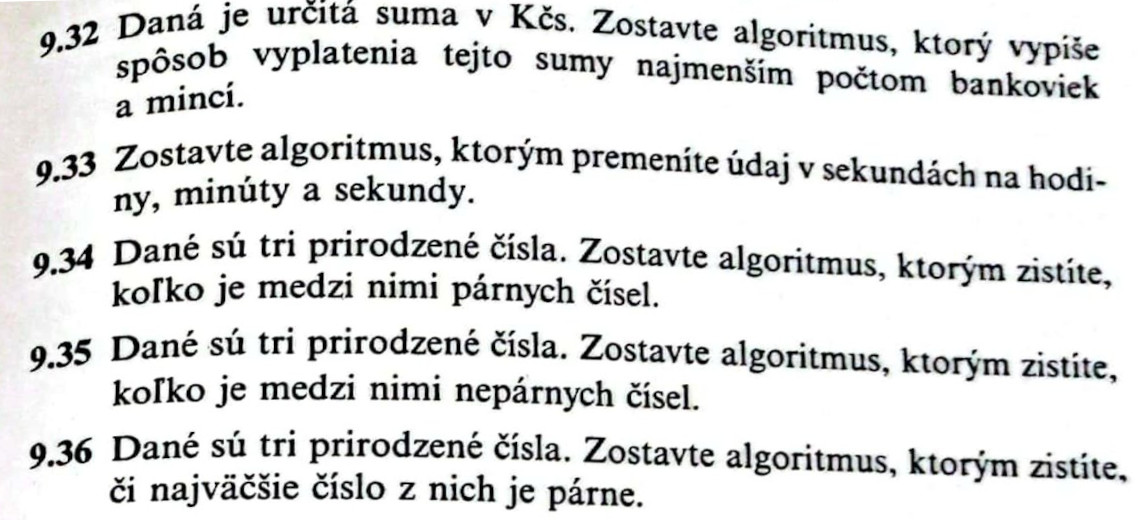
\includegraphics[width=\textwidth]{assets/zbierka-mat-vetvenie.jpg}}
\caption{Úlohy na podmienený výraz}
\end{subfigure}
\hfill
\begin{subfigure}[b]{0.48\textwidth}
\centering
\fbox{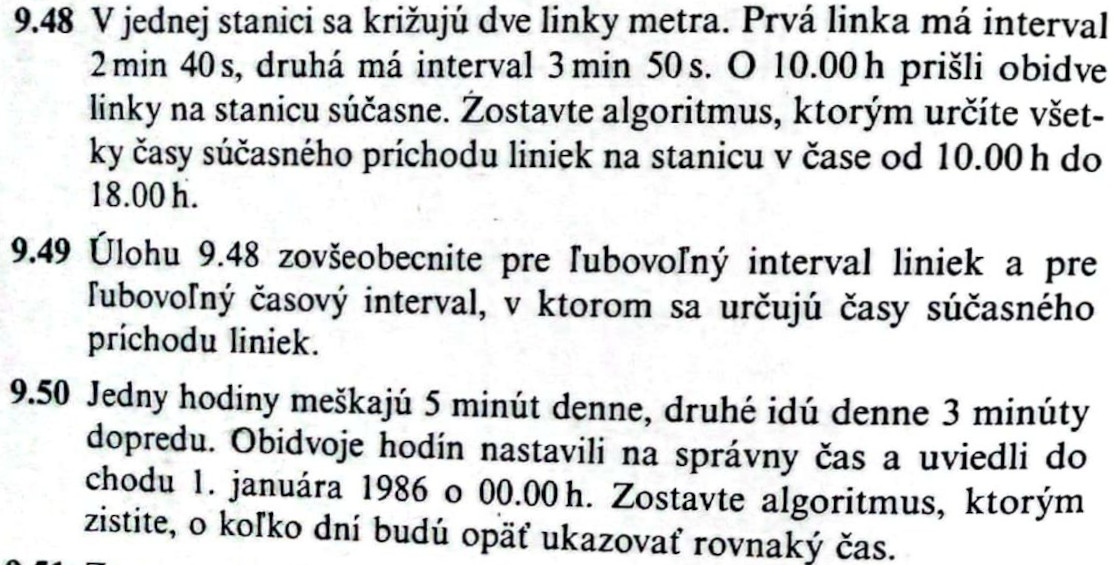
\includegraphics[width=0.9\textwidth]{assets/zbierka-mat-cyklus.jpg}}
\caption{Úlohy na príkaz cyklu}
\end{subfigure}
\caption{Ukážky z kapitoly algoritmy v zbierke úloh z matematiky pre 3. ročník~SŠ}
\label{fig:matematika-slovne-ulohy}
\end{figure}

Odlišný prístup ku grafickej úprave majú knihy zo série ,,Skúsiš to s ...'', v rámci ktorej boli uvedené knihy programovania pre mikropočítače v Basicu a strojovom kóde (\cite{tatchellova_skusis_1990}, \cite{wattsova_skusis_1991}). Cieľové miesta pôsobenia knihy neboli v čase vydania zrejme školy, ale skôr počítačové krúžky ako voľnočasové aktivity. Tieto dve knihy sa nápadite odlišujú pestrofarebnými ilustráciami až takmer komiksovým podtónom, kde sú hlavnými hrdinami roboti v ľudskom a hmyzom stvárnení a mimozemšťania. Krátke odseky výkladového textu sú obohatené o motivovanie každého príkazu jednoduchým príkladom priamo pobádajúcim na odskúšanie (Obr.~\ref{fig:skusis-prog-premenne}). Funkčné bloky kódu rozsiahlejších programov sú priebežne vysveľované textom so svorkami (Obr.~\ref{fig:skusis-prog-kozmicke-bane}), čo môže slúžiť ako dobrý model na prezentovanie riešení v zbierke.

\begin{figure}[h]
\centering
\begin{subfigure}[b]{0.55\textwidth}
\centering
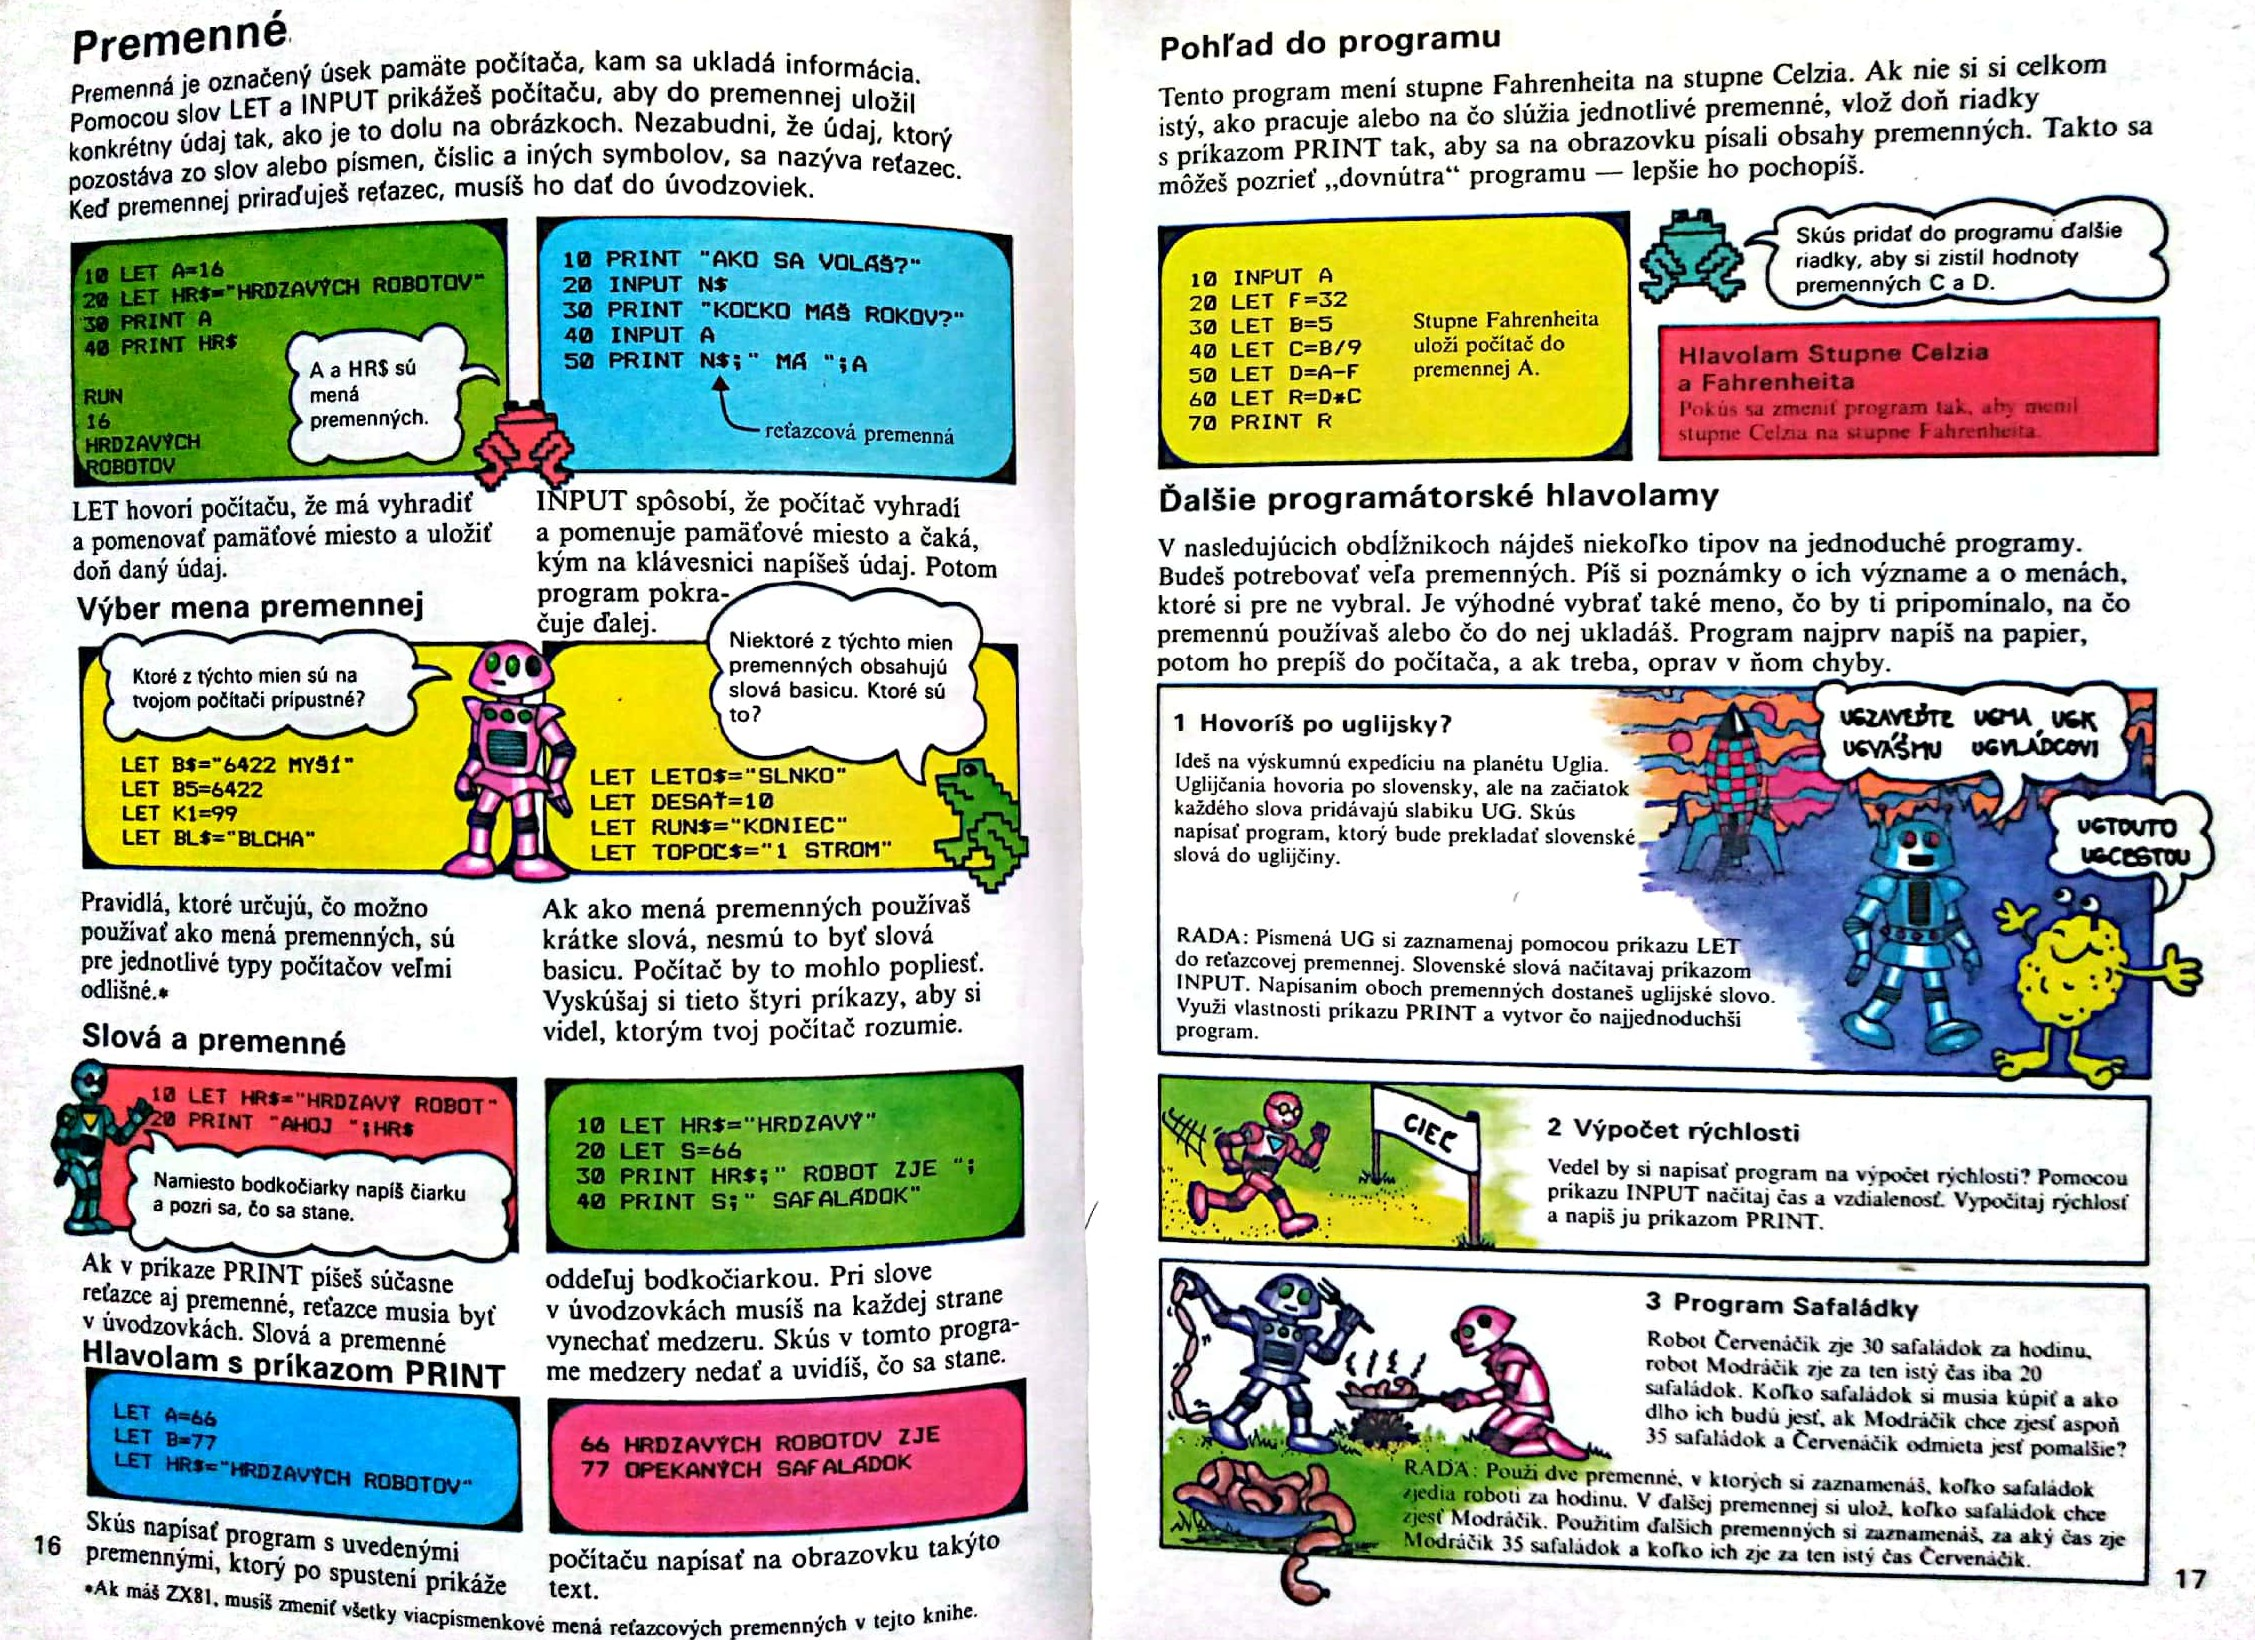
\includegraphics[width=\textwidth]{assets/kniha-premenne.jpg}
\caption{Výkladový text o premenných s hlavolamami}
\label{fig:skusis-prog-premenne}
\end{subfigure}
\hfill
\begin{subfigure}[b]{0.44\textwidth}
\centering
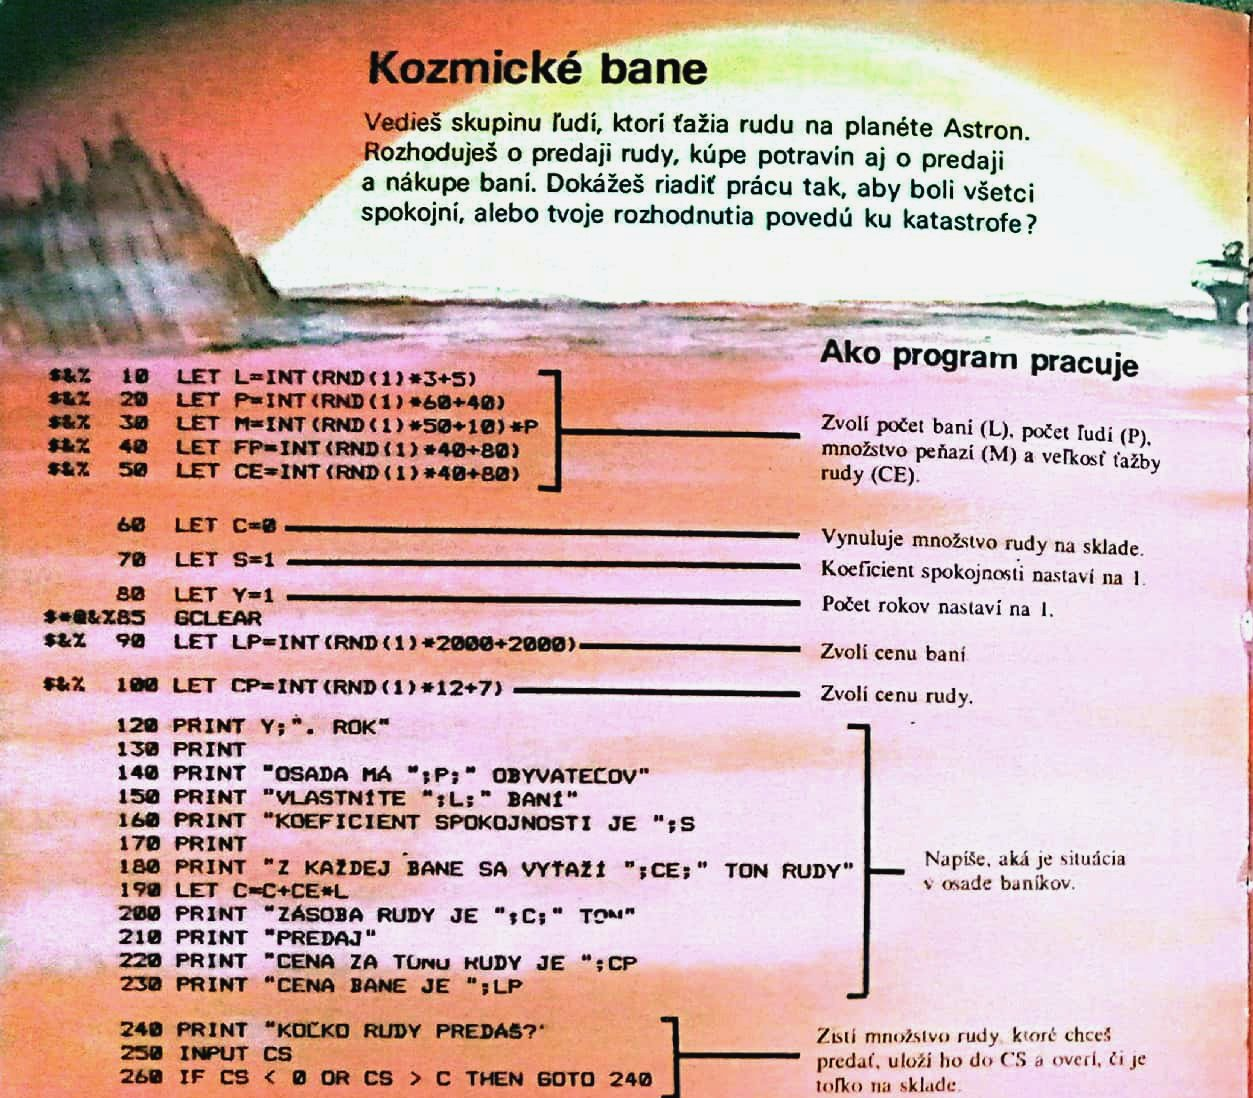
\includegraphics[width=\textwidth]{assets/program-kozmicke-bane.jpg}
\caption{Opis kódu program počítačovej hry}
\label{fig:skusis-prog-kozmicke-bane}
\end{subfigure}
\caption{Bohato ilustrovaná kniha o programovaní v jazyku Basic}
\end{figure}

Učebné texty na webe pod názvom: ,,Algoritmy a programovanie v Pascale: nielen pre maturantov z predmetu informatika'', tvoria obsiahly prierez prvkov programovacieho jazyka konkrétne: výraz s premennou, údajové typy, vetvenie, cyklus, cyklus v cykle, procedúry, funkcie, rekurzia, jednorozmerné polia, textový súbor, vyhľadávanie a triedenie polí, reťazce znakov (\cite{hedvigova_algoritmy_2007}). Učebnica je prehľadne štruktúrovaná. Z obsahu sa hypertextom smeruje na kapitoly, kde je každý nový pojem typograficky zvýraznený podčiarknutím, príkazy jazyka sú odlíšené neproporcionálnym rezom a farbou písma. Po jadre kapitoly nasledujú obvykle 2 vzorové príklady s riešeniami, spravidla 3 priebežné programátorské úlohy (Obr.~\ref{fig:uloha-pascal}), otázky na opakovanie teórie, a úlohy na precvičovanie celej témy. Na konci učebnice je umiestnených 51 jednoduchších úloh na opakovanie a 30 úloh pre náročnejších, ktorým však chýba zmysluplná organizácia náročnosti.

\begin{figure}[h]
\centering
\fbox{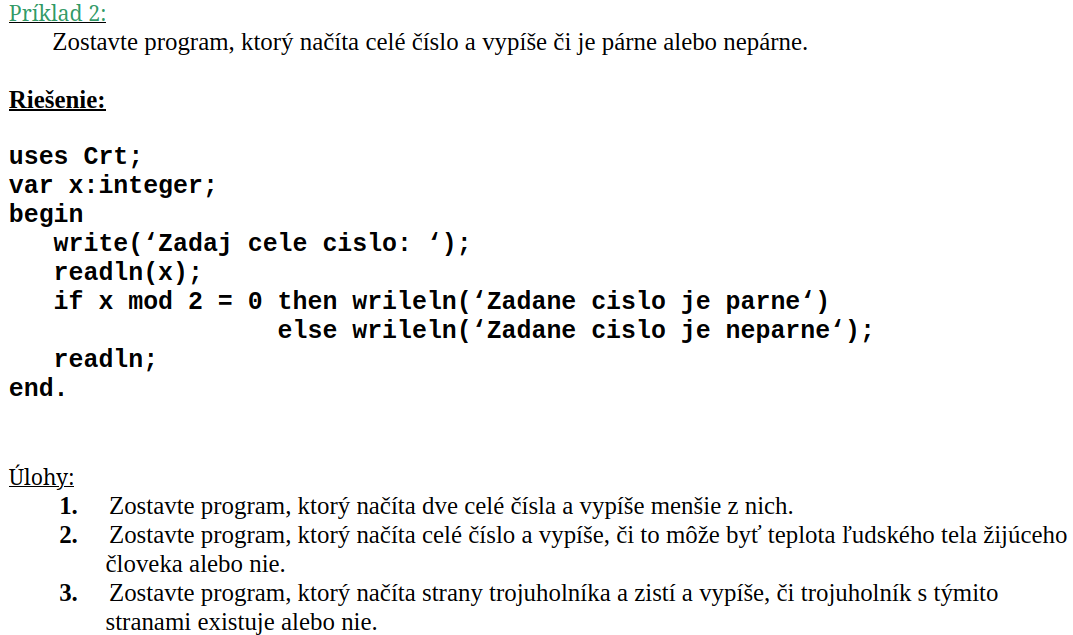
\includegraphics[width=0.7\textwidth]{assets/uloha-pascal.png}}
\caption{Riešený príklad z vetvenia nasledovaný úlohami na samostatnú prácu}
\label{fig:uloha-pascal}
\end{figure}

Slovné úlohy objasňujúci s príbehom  problémové situácie, sú prítomné v súťažiach ako sú Olympiáda v Informatike, organizovanú Národným inštitútom vzdelávania a mládeže, alebo Zenit, Korešpondenčný seminár (KSP) a Letné školy, organizované občianskym združením Trojsten. Vzorové riešenia zadaní vychádzajú v príručkách po skončení kôl. Keďže úlohy bývajú nad rámec základného učiva, tak na vysvetlenie často sa vyskytujúcich algoritmov vznikla tzv. Kuchárka KSP (\cite{noauthor_kucharka_2022}). Ukážka na Obr.~\ref{fig:ksp-oblecenie} ilustruje predlohu pre zadanie z KSP, ktorá sa vyznačuje okrem popisu situácie cez krátky dej, jasným stanovením vstupov a výstupov. 

\begin{figure}[h]
\centering
\fbox{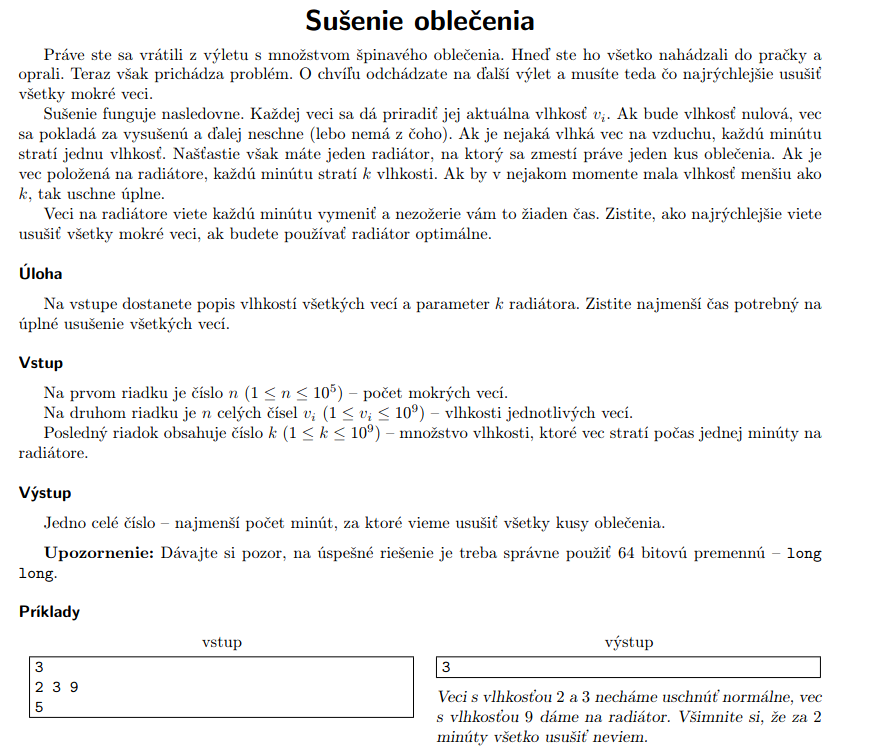
\includegraphics[width=0.7\textwidth]{assets/susenie-oblecenia.png}}
\caption{Úloha letnej školy KSP na binárne vyhľadávanie s úvodným príbehom}
\label{fig:ksp-oblecenie}
\end{figure}

Uvedenie programovacieho jazyka \emph{Python} do výučby informatiky na stredných školách znamenal dopyt po nových učebných materiáloch, ktoré preložia zápisy hlavne z dosiaľ používaného jazyku Pascal. Medzi učebnicami Pythonu prevláda trend predstavovať programovanie cez procedurálne kreslenie cez modul \emph{tkinter}, \emph{turtle}, niekedy \emph{pygame}. V grafickom programovaní sa pojem cyklu prestavuje oveľa skorej ako podmienky, presne naopak než v textovom móde.

Kučera a Výbošťok dali dohromady trojdielnu sériu učebníc ,,Programujeme v Pythone'', v slovenskom a anglickom jazyku so zodpovedajúcimi príručkami pre učiteľov a testami k učebnici. Vypracovali aj zbierku 64 riešených úloh k maturite z informatiky ,,Maturujeme v Pythone''. Vychádzali z potrieb aktívnych učiteľov z Klubu učiteľov vedeného autorom. Osnova prvého diela učebnice začína grafickými príkazmi (Obr.~\ref{fig:kucera-kreslenie-python}) a ďalej sa skladá z premenných, opakovaní častí programu, podprogramov, klikania myšou a ovládaním klávesnicou, podmienených príkazov, časovača a snaženie sa zavŕši tvorbou jednoduchých hier (\cite{kucera_programujeme_2016}). 

\begin{figure}[h]
\centering
\begin{subfigure}[b]{0.55\textwidth}
\centering
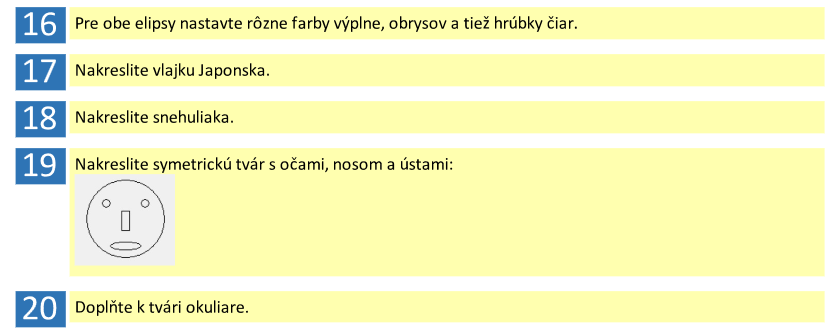
\includegraphics[width=\textwidth]{assets/kucera-python.png}
\caption{Kreslenie obdĺžníkov}
\label{fig:kucera-kreslenie-python}
\end{subfigure}
\begin{subfigure}[b]{0.44\textwidth}
\centering
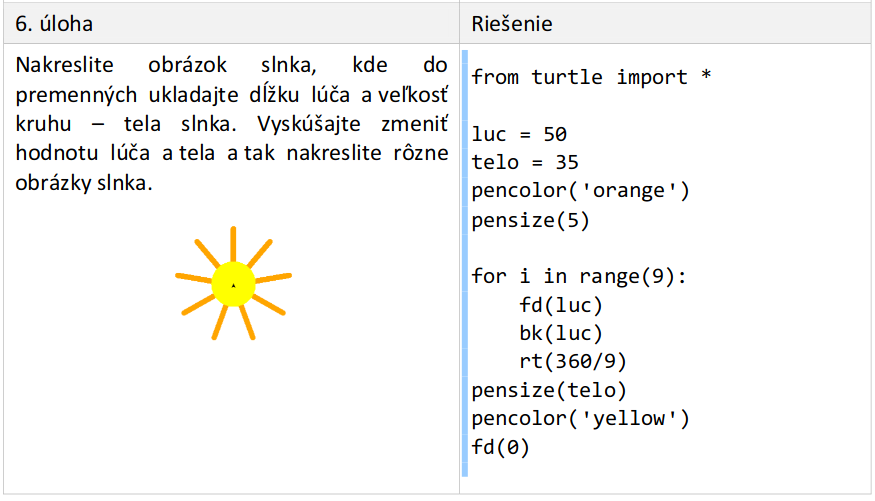
\includegraphics[width=\textwidth]{assets/uloha-turtle.png}
\caption{Cyklus a korytnačia grafika}
\label{fig:turtle-graphics}
\end{subfigure}
\caption{Úlohy na programovanie grafiky v jazyku Python}
\end{figure}

Blaho a Salanci pripravili pracovné listy \emph{abcPython} na 20 vyučovacích hodín, kde nepočítajú s výkladom učiteľa. Dostupné sú aj metodické materiály ku listom. Preberajú sa postupne témy kde sa prelína textový a grafický režim: interaktívny zadávanie príkazov, výrazy, premenné, výpisy, kreslenie, náhoda, výrazy v cykle, elipsy, vetvenie, podprogramy, kreslenie myšou (\cite{blaho_abcpython_2019}, \cite{blaho_metodiky_2019}). 

Mészárosová vytvorila metodickú príručku pre vyučovanie základov programovania, kde cez Python rozvíja na rozpätí 16 vyučovacích hodín korytnačiu grafiku (Obr.~\ref{fig:turtle-graphics}). Využíva tým oboznámenosť žiakov s korytnačkami v jazyku Logo z druhého stupňa základnej školy. Rovnako sa začína predstavením grafickými pokynov na pohyb a kreslenie korytnačkou. Nasledujú premenné, for cyklus, funkcie, funkcie s parametrami, poloha korytnačky, náhodná poloha, vetvenie a na upevnenie zručností slúži projekt kreslenia pohľadnice (\cite{meszarosova_python_2017}).

